\section{Case Study: Key-Value Store}
\label{sec:kvs}
The next two sections contain case studies that show how \lang can be used to
build practical distributed programs.\footnote{Complete code listings for these
  case studies are available at \mbox{\small
    \url{http://db.cs.berkeley.edu/bloom-lattice}}.} Both case studies are
monotonic: that is, both programs consist of monotone functions applied to
lattices. As a result, the \lang compiler can verify that both of them are
eventually consistent without any need for coordination.

In the first case study, we show that a distributed, eventually consistent
key-value store can be \emph{composed} via a series of monotonic mappings
between simple lattices. This example shows how \lang overcomes
the ``scope dilemma'' of CvRDTs: by composing a complex program from simple
lattices (mostly \lang built-ins), we can feel confident that individual
lattices are correct, while CALM analysis finishes the job of verifying
whole-program correctness.

%  This
% demonstrates that \lang's built-in lattices are useful and yields a very concise
% implementation. Morever, using lattice composition gave us confidence in the
% correctness of our code, because much of the program's complexity resides in
% simple built-in lattices that we 

%  More importantly, composing a complex program from simple
% lattices made it easy to reason about the behavior of the entire program

%  and results in a very
% concise implementation. Moreover, it gives us confidence in the correctness of
% our implementation, because much of the program's complexity is handled by the
% behavior of the built-in lattices, which are likely to be correct.  \paa{not
%   sure what to suggest, but this last clause seems underconfident (and slightly
%   run-on).  perhaps we just want to say that we assert them to be correct, or
%   that it's easy to prove/convince ourselves that they are correct due to their
%   simplicity, etc}

\subsection{Basic Architecture}
\begin{figure}[t]
\begin{scriptsize}
\begin{lstlisting}
module KvsProtocol
  state do
    channel :kvput, [:reqid, :@addr] => [:key, :val,
                                         :client_addr]
    channel :kvput_resp, [:reqid] => [:@addr, :replica_addr]
    channel :kvget, [:reqid, :@addr] => [:key, :client_addr]
    channel :kvget_resp, [:reqid] => [:@addr, :val,
                                      :replica_addr]
  end
end
\end{lstlisting}
\end{scriptsize}
\caption{Key-value store interface.}
\label{fig:kvs-interface}
\end{figure}

\begin{figure}[t]
\begin{scriptsize}
\begin{lstlisting}
class KvsReplica
  include Bud
  include KvsProtocol

  state { lmap :kv_store } (*\label{line:kvs-map-ddl}*)

  bloom do
    kv_store   <= kvput {|c| {c.key => c.val}} (*\label{line:kvs-put-merge}*)
    kvput_resp <~ kvput {|c| [c.reqid, c.client_addr, ip_port]}
    kvget_resp <~ kvget {|c| [c.reqid, c.client_addr,
                              kv_store.at(c.key), ip_port]}
  end
end
\end{lstlisting}
\end{scriptsize}
\caption{KVS replica implementation in \lang.}
\label{fig:kvs-replica}
\end{figure}

A key-value store (KVS) provides a lookup service that allows client
applications to store and retrieve the \emph{value} associated with a given
\emph{key}. Key-value pairs are typically replicated on multiple storage nodes
for redundancy and the key space is partitioned to improve aggregate storage and
throughput. \emph{Eventual consistency} is a common correctness criterion: after
all client updates have reached all storage nodes, all the replicas of a
key-value pair will converge to the same final state~\cite{Terry1995,vogels}.

Figure~\ref{fig:kvs-interface} shows a simple KVS interface in \lang. Client
applications initiate \emph{get(key)} and \emph{put(key, val)} operations by
inserting facts into the \texttt{kvget} and \texttt{kvput} channels,
respectively; server replicas return responses via the \texttt{kvget\_resp} and
\texttt{kvput\_resp} channels.

Figure~\ref{fig:kvs-replica} contains the \lang code for a KVS server
replica. An \texttt{lmap} lattice is used to maintain the mapping between keys
and values (line~\ref{line:kvs-map-ddl}). Since the values in an \texttt{lmap}
lattice must themselves be lattice elements, for now we assume that clients only
want to store and retrieve monotonically increasing lattice values; we discuss
how to lift this restriction in Section~\ref{sec:kvs-versions}. To handle a
\emph{put(key, val)} request, a new \emph{key} $\to$ \emph{val} \texttt{lmap} is
created and merged into \texttt{kv\_store} (line~\ref{line:kvs-put-merge}). If
\texttt{kv\_store} already contains a value for the given key, the two values
will be merged together using the value lattice's merge function (see
Section~\ref{sec:lattice-built-ins} for details). Observe that we use the \lang
features described in Section~\ref{sec:bloom-interop} to allow traditional Bloom
collections (e.g., channels) and lattices (e.g., the \texttt{kv\_store} lattice)
to be used by the same program. Note also that \texttt{ip\_port} is a built-in
function that returns the IP address and port number of the current Bud
instance.

The state of two replicas can be synchronized by simply exchanging their
\texttt{kv\_store} maps; the \texttt{lmap} merge function automatically resolves
conflicting updates made to the same key. This property allows considerable
flexibility in how replicas propagate updates.
% TODO: (1) finish repl discussion (composition, replication strat) (2) partitioning

\subsection{Object Versioning}
\label{sec:kvs-versions}
\begin{figure}[t]
\centering
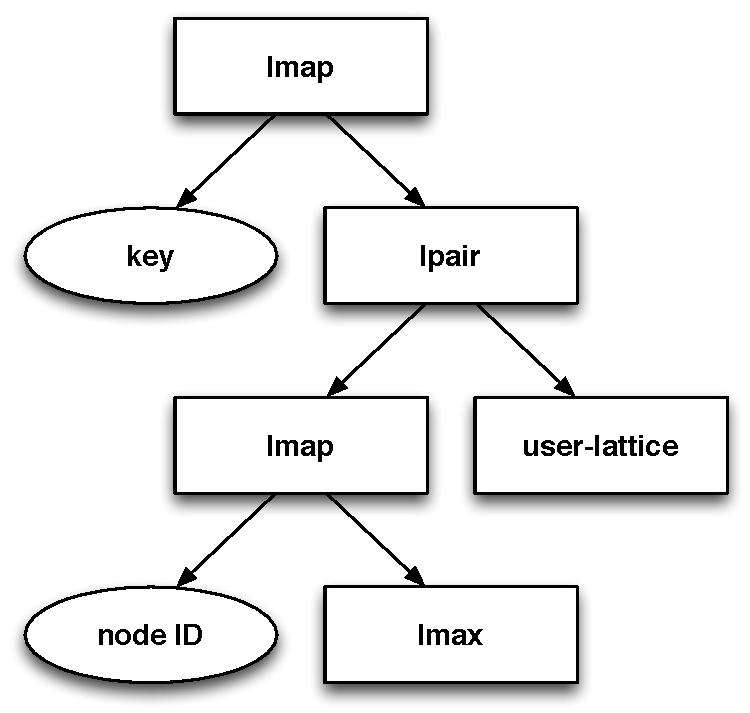
\includegraphics[width=0.8\linewidth]{fig/kvs-vc-lattice.pdf}
\caption{Lattice structure of a KVS with object versioning. Rectangles are
  lattices and ovals are atomic values.}
\label{fig:kvs-vc-lattices}
\end{figure}

The basic KVS design is sufficient for applications that want to store
monotonically increasing values such as session logs or increasing counters. To
allow storage of values that change in arbitrary ways, we now consider how to
support \emph{object versions}. This is a classic technique for recognizing and resolving
mutual inconsistency between members of a distributed system~\cite{Parker1983}.
Our design is similar to that used by Amazon Dynamo~\cite{DeCandia2007}.

Each replica associates keys with sets of
$\langle\textit{vector-clock},\textit{value}\rangle$ pairs. The vector clock
captures the causal relationship between different versions of a
record~\cite{Fidge1988,Mattern1989}. Clients store and retrieve
$\langle\textit{vector-clock},\textit{value}\rangle$ pairs. When a client
updates a value it has previously read, the client increments its own position
in the vector clock and includes the updated vector clock $V_U$ with its
\emph{put} operation. Upon receiving an update, the server compares $V_U$ with
the set of vector clocks associated with the updated key. For each such vector
clock $V_S$, the server considers three cases:
\begin{compactenum}
\item $V_U > V_S$: the client's update happens-after $V_S$, so $V_S$ is replaced
  with $V_U$.
\item $V_U < V_S$: the client's update happens-before $V_S$, so $V_S$ is
  retained.\footnote{This situation might arise due to duplication and
    reordering of messages by the network.}
\item $V_U$ and $V_S$ are incomparable: the two versions are concurrent, so
  both $V_U$ and $V_S$ are retained.
\end{compactenum}
By applying these rules, each replica retains a set of mutually concurrent
versions for each key. To handle a \emph{get} operation, the server returns a
single $\langle\textit{vector-clock},\textit{value}\rangle$ pair by merging
together the vector clocks and using a user-supplied reconciliation function to
merge together the conflicting values, as described below. We call the set of
incomparable version-value pairs a \emph{dominating set}.

From a \lang perspective, each replica still stores a monotonically increasing
value---the only difference is that in this scheme, the \emph{version} stored by
a replica increases over time, rather than the associated value. Hence, we now
consider how to support vector clocks and dominating sets using \lang.

\subsubsection{Vector Clocks}
A vector clock is a map from node identifiers to logical
clocks~\cite{Fidge1988,Mattern1989}. Let $V_e$ denote the vector clock for event
$e$; let $V_e(n)$ denote the logical clock associated with node $n$ in $V_e$. If
$V_e < V_{e'}$, $e$ causally precedes $e'$, where
\begin{displaymath}
V_e < V_{e'} \equiv \forall x [ V_e(x) \leq V_{e'}(x) ] \land \exists y [ V_e(y) < V_{e'}(y) ]  
\end{displaymath}
In \lang, a vector clock can be represented as an \texttt{lmap} that maps node
identifiers to \texttt{lmax} values. Each \texttt{lmax} represents the logical
clock of a single node; this is appropriate because the logical clock value
associated with a given node will only increase over time. The merge function
provided by \texttt{lmap} achieves the desired semantics---that is, the built-in
least upper bound for an \texttt{lmap} that contains \texttt{lmax} values is
consistent with the partial order given above.\footnote{The observation that
  vector time has a lattice structure was made by Mattern~\cite{Mattern1989}.}

\subsubsection{Dominating Sets}
We use a custom lattice type \texttt{ldom} to represent a dominating set. As
discussed above, a dominating set is a set of
$\langle\textit{version},\textit{value}\rangle$ pairs; both elements of the pair
are themselves represented as lattice values. In the KVS, the version lattice is
a vector clock (that is, an \texttt{lmap} containing \texttt{lmax} values); the
value lattice is whatever value the user wants to store in the KVS.\footnote{If
  the user stores a value that does not have a natural merge function, similar
  systems typically provide a default merge function that collects conflicting
  updates into a set for eventual manual resolution by the user. Such a strategy
  corresponds to using \texttt{lset} as the value lattice in \lang.}

The discussion above suggests a natural merge function for \texttt{ldom}: given
two input \texttt{ldom} elements $e$ and $e'$, the merge function omits all
``dominated'' pairs. For example, a
$\langle\textit{version},\textit{value}\rangle$ pair in $e$ is included in the
result of the merge unless there is a pair in $e'$ whose version is strictly
greater.

The \texttt{ldom} lattice provides two functions, \texttt{version} and
\texttt{value}, that return the least upper bound of the concurrent versions or
values, respectively. In the KVS, the \texttt{value} function corresponds to
reconciling conflicting updates, whereas \texttt{version} returns the vector
clock associated with the reconciled value. Note that while the \texttt{version}
of a given \texttt{ldom} increases over time (as new versions are observed), the
\texttt{value} does not; hence, \texttt{version} is a monotone function but
\texttt{value} is not. Since the goal of object versioning is to allow values to
change in non-monotonic ways, this is the expected behavior.

\subsubsection{Discussion}
Figure~\ref{fig:kvs-vc-lattices} shows the lattices used in a KVS with object
versioning. Surprisingly, adding support for object versioning did not require
\emph{any} changes to the KVS replica code. Instead, clients simply store
\texttt{ldom} values containing a single
$\langle\textit{vector-clock},\textit{value}\rangle$ pair, incrementing their
position in the vector clock as described above. The KVS replica merges these
\texttt{ldom} values into an \texttt{lmap} as usual; the merge function of
\texttt{ldom} handles conflict resolution in the appropriate manner. Moreover,
by composing the KVS from a collection of simple lattices, we found it easy to
reason about the behavior of the system. For example, convincing ourselves that
KVS replicas will eventually converge only required checking that the individual
\texttt{ldom}, \texttt{lmap}, and \texttt{lmax} lattices satisfy the lattice
properties, rather than analyzing the behavior of the system as a whole.

Our design compares favorably to traditional implementations of object
versioning and vector clocks. For example, the implementation of vector clocks
alone in the Voldemort KVS requires 216 lines of Java, not including whitespace
or comments~\cite{voldemort-vector-clock}. In \lang, vector clocks follow
directly from the composition of the \texttt{lmap} and \texttt{lmax} lattices,
and the \emph{entire KVS} requires less than 100 lines of Ruby and \lang code,
including the client library. The \texttt{ldom} lattice requires an additional
50 lines of Ruby but is completely generic, and could be included as a built-in
lattice.

\subsection{Quorum Reads and Writes}
To further demonstrate the flexibility of our implementation, we add an
additional feature to our KVS: the ability to submit reads and writes to a
configurable number of nodes. If a client reads from $R$ nodes and writes to $W$
nodes in a KVS with $N$ replicas, the user can set $R + W > N$ to achieve
behavior equivalent to a quorum replication system~\cite{Gifford1979}, or use
smaller values of $R$ and $W$ if eventual consistency is sufficient. This scheme
allows users to vary $R$ and $W$ on a per-operation basis, depending on their
consistency, durability, and latency requirements.

To support this feature, we can use the \lang quorum voting pattern
introduced in Figure~\ref{fig:lattice-quorum}. After sending a write to $W$
systems, the KVS client accumulates \texttt{kvput\_resp} messages into an
\texttt{lset}. Testing for quorum can be done in a monotonic fashion by mapping
the \texttt{lset} to an \texttt{lmax} (using the \texttt{size} method) and then
performing a threshold test using \texttt{gt\_eq} on \texttt{lmax}. As expected,
this is monotonic: once quorum has been reached, it will never be retracted.

Quorum reads work similarly except that the client must also merge together the
$R$ versions of the record it receives. This follows naturally from the
discussion in Section~\ref{sec:kvs-versions}: the client simply takes the least
upper bound of the values it receives, which produces the expected behavior. The
client can optionally write the merged value back to the KVS (so-called ``read
repair''~\cite{DeCandia2007}); note that the \texttt{ldom} merge method also
updates the record's vector clock appropriately.
